\chapter{Introdução}

Os alunos sempre acabam perdendo muito tempo somente formatando suas monografias e dissertações nos padrões malucos da ABNT e da EEL. Digo este 'e' porque a formatação da EEL usa somente em parte as normas da ABNT (vai entender porque), e pra descobrir quando usar uma ou outra pode ser trabalhoso e até estressante. Como já passei por isto, decidi usar a minha dissertação de mestrado como modelo, nos padrões que foram aceitos na biblioteca da EEL, com a intenção de ajudar os futuros alunos com suas respectivas dissertações ou monografias. 

Este template não aborda todos os padrões, somente os que foram mais essenciais que eu acabei usando. Não acredito que seja necessário usar muito mais do que há neste modelo, mas sintam-se a vontade para atualizar este documento, este é somente o ponto de partida. 

Os pacotes de formatação já estão todos adicionados, basta colocar o seu texto, figuras e tabelas nos locais apropriados e ser feliz! 

\begin{figure}
	\centering
	\caption{Exemplo de uma figura.}
	
\includegraphics[width=0.6\textwidth]{Got}
	\label{Selecione_um_label_para_chamar_no_texto_com_o_comando_ref{}.}
	\raggedright
	\caption*{Fonte: adaptado de Fullretard}
\end{figure}


\begin{figure}
	\centering
	\caption{Exemplo de figuras lado a lado.}
	\begin{subfigure}[t]{0.5\textwidth}
		\caption{Wolverine}
		\centering
		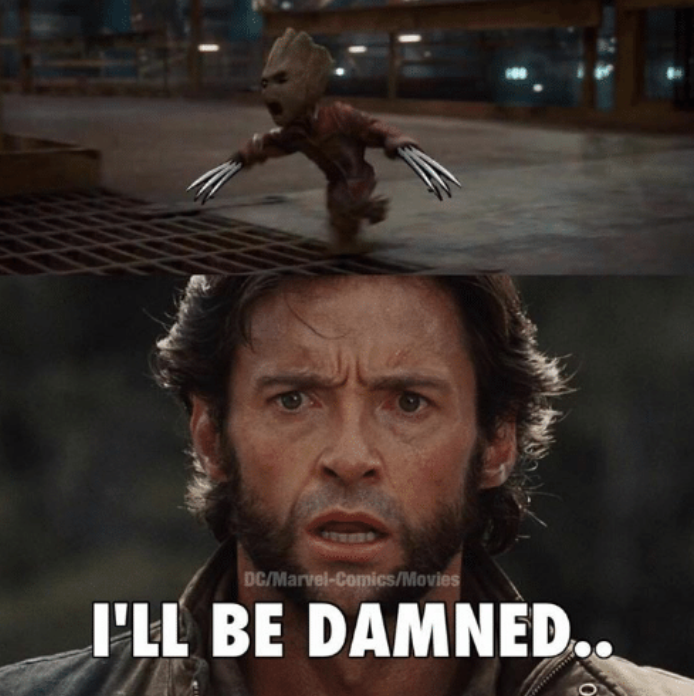
\includegraphics[width=\linewidth]{Wolverine}
	\end{subfigure}%\hskip 1em%
	\begin{subfigure}[t]{0.5\textwidth}
		\caption{Marvel}
		\centering
		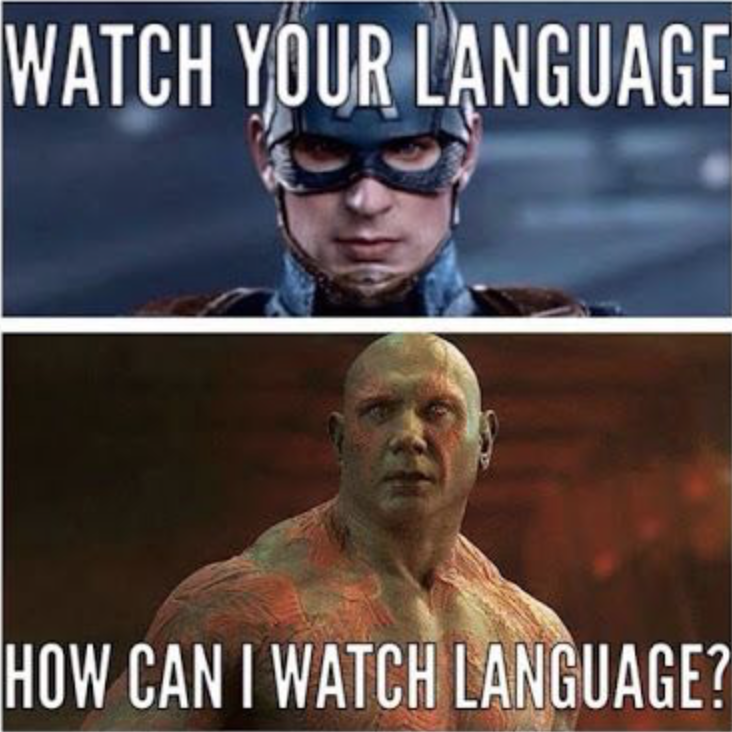
\includegraphics[width=\linewidth]{Drax}
	\end{subfigure}
	\begin{subfigure}[t]{0.5\textwidth}
		\caption{Dark Knight}
		\centering
		
\includegraphics[width=\linewidth]{Coringa}
	\end{subfigure}%\hskip 1em%
	\begin{subfigure}[t]{0.5\textwidth}
		\caption{Interstellar}
		\centering
		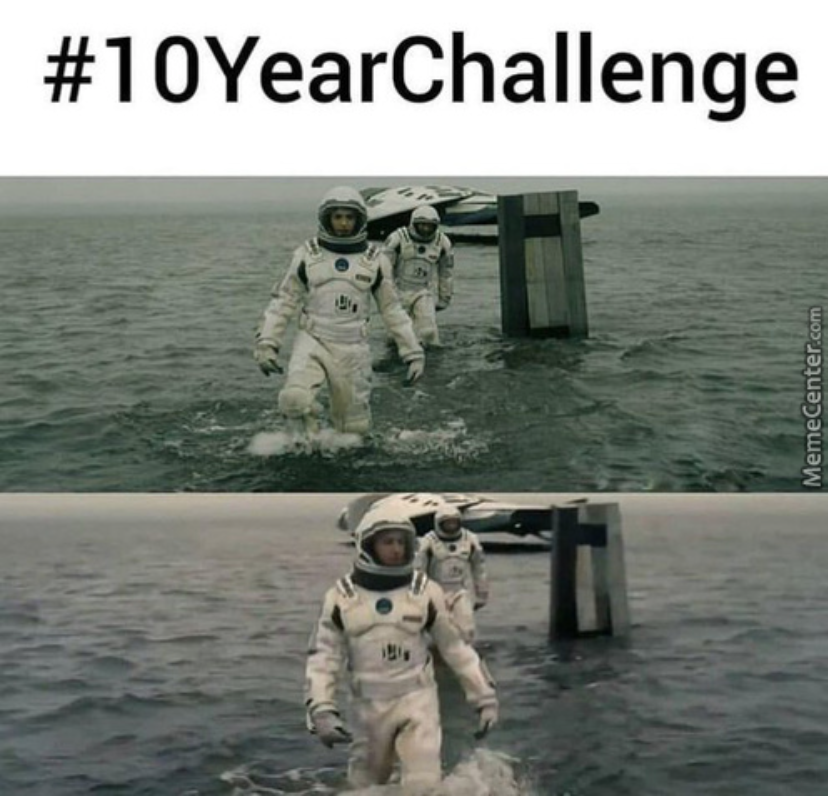
\includegraphics[width=\linewidth]{Interstelar}
	\end{subfigure}
	
	\begin{subfigure}[t]{0.5\textwidth}
		\caption{Inception}
		\centering
		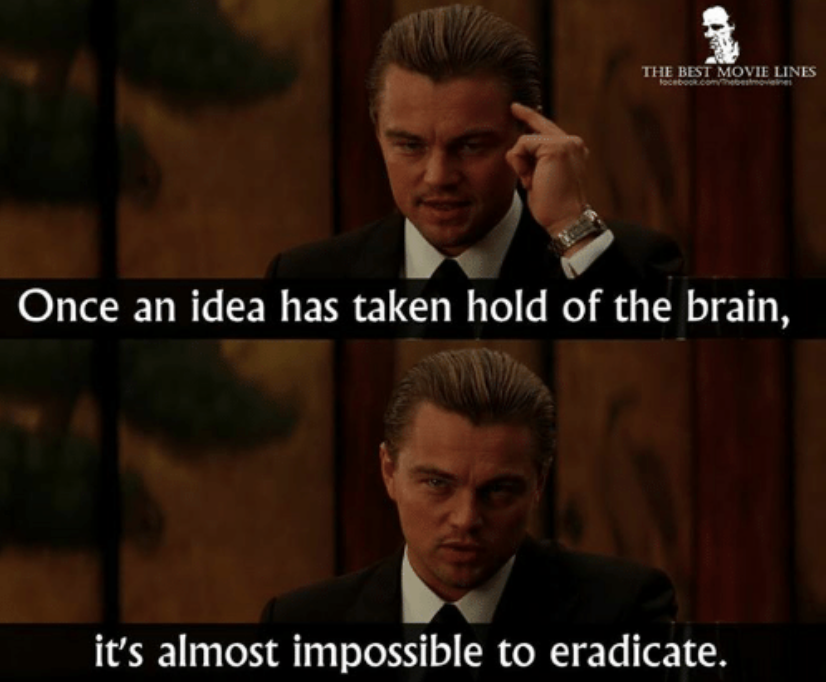
\includegraphics[width=\linewidth]{Leo}
	\end{subfigure}%\hskip 1em%
	\begin{subfigure}[t]{0.5\textwidth}
		\caption{The hateful eight}
		\centering		
		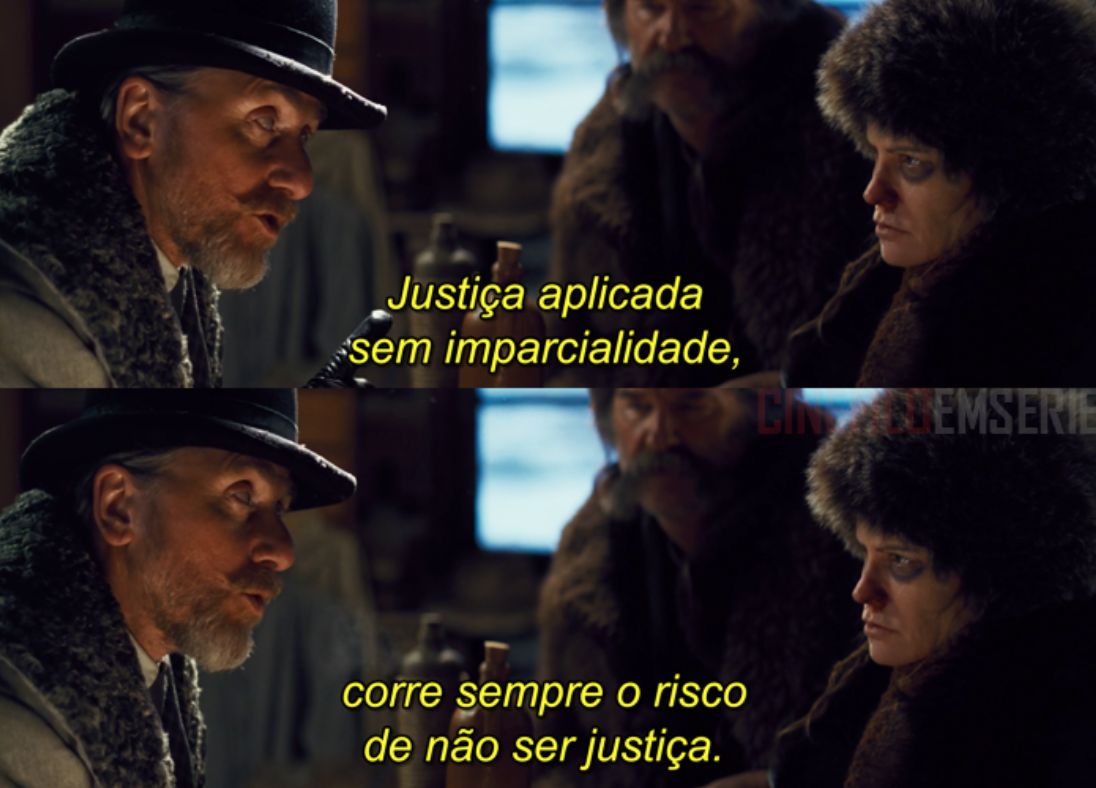
\includegraphics[width=\linewidth]{Odiados}
	\end{subfigure}
	\label{fig:mev1}
	\caption*{Fonte: autor}
	\caption*{Nota: Memes de filmes que valem a pena assistir.}
\end{figure}

\begin{table}
	\centering
	\caption{Exemplo de tabela com referências.}
	\begin{tabular}{ccc}
		\toprule
		Referências & $\Delta_f$H & Método\\
		\midrule
		\cite{Kleppa1998} & -33,6 & Calorimetria de síntese\\
		\cite{Eremenko1972} & -34,4 & Extrapolação (EMF)\\
		\cite{Lukashenko1986} & -34,8 & Extrapolação (EMF)\\
		\cite{Chart1975} & -27,9 & Efusão de Knudsen\\
		\cite{deBoer1982} & -31,0 & Estimativa (Miedema)\\
		\cite{Coughanowr1994} & -32,5 & Calculado (CALPHAD)\\
		\cite{Schuster2000} & -32,5 & Calculado (CALPHAD)\\
		\bottomrule
		
	\end{tabular}
	\label{tab:T1-entalpias}
	\caption*{Fonte: autor}
\end{table}

Equação simples:

\begin{equation}
\centering
\hat{H}\psi=E\psi
\label{Schro}
\end{equation}

Equação mais complicada:

\begin{multline}
\bigg[\overbrace{-\frac{\hbar}{2m_{i}}\sum_i\nabla_i^2}^{\hat{T}} +\overbrace{\frac{e^2}{4\pi\epsilon_0}\sum_j\sum_{j'>j}\frac{Z_jZ_{j'}}{|\vec{R}_j-\vec{R}_{j'}|}}^{\hat{V}_{NN}} -\overbrace{\frac{e^2}{4\pi\epsilon_0}\sum_i\sum_{j}\frac{Z_j}{|\vec{r}_i-\vec{R}_{j}|}}^{\hat{V}_{eN}} \\ +\underbrace{\frac{e^2}{4\pi\epsilon_0}\sum_i\sum_{i'>i}\frac{1}{|\vec{r}_i-\vec{r}_{i'}|}}_{\hat{V}_{ee}}\bigg]\Psi = E_{tot}\Psi
\end{multline}

\begin{figure}[h]
	\centering
	\caption{Exemplo do pacote tikz.}
	\tikzstyle{decision} = [diamond, draw, text width=7em, text centered, node distance=5cm, inner sep=0pt]
	\tikzstyle{block} = [rectangle, draw, text width=9em, text centered, rounded corners, minimum height=4em]
	\tikzstyle{line} = [draw, -latex']
	\begin{tikzpicture}[node distance = 5cm, auto]
	\node [block] (init) {Densidade inicial (estimativa) $\rho(\vec{r})$};
	\node [block, right of = init] (Kohn-Sham) {Resolver as equações de Kohn-Sham};
	\node[right of = Kohn-Sham] (step) {};
	\node [block, below of = step] (Electron-Density) {Energia $E$, nova densidade $\rho(\vec r)$};
	\node [decision, left of = Electron-Density] (Erro) {Energia convergiu?};
	\node [block, left  of = Erro] (convergido) {$E$ e $\rho(\vec{r})$ finais};
	\path [line] (init) -- (Kohn-Sham);
	\path [line] (Kohn-Sham) -| (Electron-Density);
	\path [line] (Electron-Density) -- (Erro);
	\path [line] (Erro) -- node {não} (Kohn-Sham);
	\path [line] (Erro) -- node {sim} (convergido);
	\end{tikzpicture}
	\label{SCF}\\
	\caption*{Fonte: \cite{Dorini2017}}
\end{figure}

\begin{figure}
	\centering
	\caption{Exemplo da aplicação do pacote \textit{minipage}.}
	\begin{minipage}{.4\textwidth}
		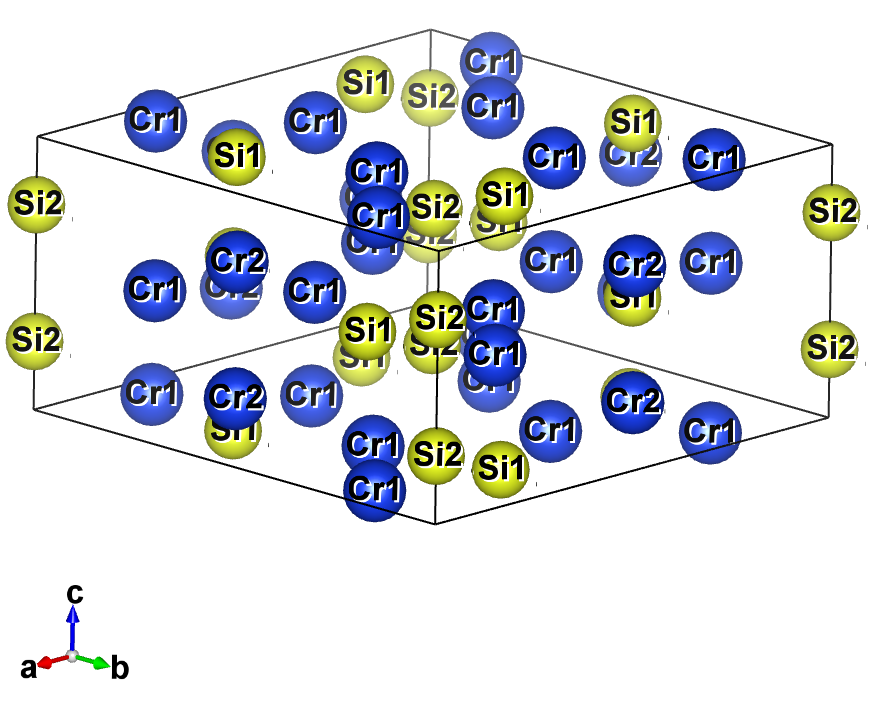
\includegraphics[width=\textwidth]{T1}
	\end{minipage}
	\begin{minipage}{.5\textwidth}
		\begin{tabular}{ll}
			%            Composto: & $\alpha$Cr$_5$Si$_3$ \\
			Grupo espacial: & $I4/mcm$ (\#140)\\
			Símbolo de Pearson: & $tI32$\\
			Protótipo: & W$_5$Si$_3$\\
			Parâmetros de rede: & $a=b=9,14\,$\AA ;  $c=4,64\,$\AA \\
			%            Posições atômicas:
		\end{tabular} \\
		% 
		\begin{tabular}{ccccccc}
			\toprule
			& Sítio & Wyckoff & Sim. & $x$ & $y$ & $z$     \\
			\midrule
			\tikz\draw[black,fill=blue!70] (0,0) circle (.7ex); & Cr1 & $16k$ & $m..$ & 0,074 & 0,223 & 0 \\
			\tikz\draw[black,fill=blue!70] (0,0) circle (.7ex); & Cr2 & $4b$ & $-42m$ & $0$ & $1/2$ & $1/4$ \\
			\tikz\draw[black,fill=yellow!70] (0,0) circle (.7ex); & Si1 & $8h$ & $m.2m$ & 0,17 & 0,67 & 0 \\
			\tikz\draw[black,fill=yellow!70] (0,0) circle (.7ex); & Si2 & $4a$ & $422$ & $0$ & $0$ & $1/4$ \\
			\bottomrule
		\end{tabular}
		%         (Hf: cinza claro; V: branco; Ga: cinza escuro)
	\end{minipage}
	\label{estrutura-T1}\\
	\caption*{Fonte: autor}
	\caption*{Nota: Adaptado de \cite{Kuzma1982}}
\end{figure}

\begin{figure}
	\centering
	\caption{Exemplo do pacote \textit{subfig} para ajustar duas figuras lado a lado.}
	\begin{subfigure}[t]{0.5\textwidth}
		\caption{}
		\centering
		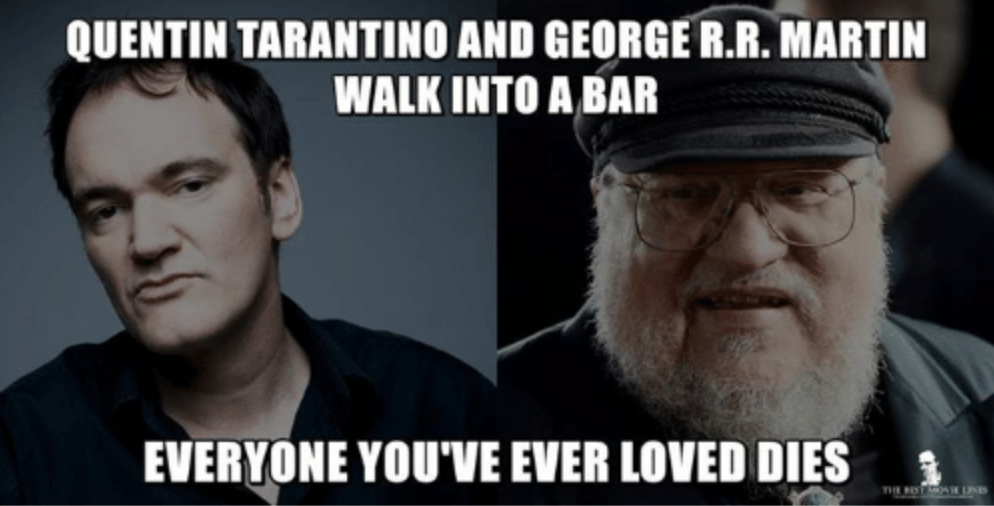
\includegraphics[width=\linewidth]{Tarantino}
	\end{subfigure}%\hskip 1em%
	\begin{subfigure}[t]{0.45\textwidth}
		\caption{}
		\centering
		
\includegraphics[width=\linewidth]{fullretard.jpg}
	\end{subfigure}
	\label{phd-crsi}
	\caption*{Fonte: autor}
\end{figure}

\begin{table}
	\centering
	\caption{Exemplo do pacote \textit{adjustbox} (que coloca o comprimento da tabela igual ao do texto, isso é muito útil!). Note que é necessário usar o \textit{top, mid e bottomrule} para diferenciar a espessura das linhas}
	\begin{adjustbox}{max width=\textwidth}
		\begin{tabular}{c|ccccc}
			& Composição& Símbolo de &Grupo &Designação & \\
			Fase &\%at. Si & \textit{Pearson} &espacial &\textit{Strukturbericht} &Protótipo \\
			\toprule
			(Cr) & 0 a 9,5 & $cI2$ & $Im-3m$& $A2$&W\\
			\hline
			(Si) & \~ 100 & $cF8$ & $Fd-3m$ & $A4$ & C (diamante) \\ 
			\hline
			Cr$_3$Si & 22,5 a 26,4 & $cP8$ & $Pm-3n$ & $A15$ & Cr$_3$Si\\
			\hline
			$\alpha$-Cr$_5$Si$_3$ & 36 a 41 & $tI32$ & $I4/mcm$& $D8_m$ & W$_5$Si$_3$\\
			\hline
			$\beta$-Cr$_5$Si$_3$ & --- & --- & --- & --- & --- \\
			\hline
			CrSi & 50 & $cP8$ & $P2_13$ & $B20$ & FeSi\\
			\hline
			CrSi$_2$ & 66,7 a 67 & $hP9$ & $P6_222$ & $C40$ & CrSi$_2$\\
			\bottomrule
		\end{tabular}
	\end{adjustbox}
	\label{tab:estruturas-cristalinas-Cr--Si}
	\caption*{Fonte: autor}
	\caption*{Nota: adaptado de \cite{Gokhale1987}}
\end{table}

Exemplo de itens:

\begin{enumerate}
	\item Texto 1
	\item Texto 2
	\item Texto 3
\end{enumerate}

